\section{Introduction}
\subsection{Finance as a science}
Finance
- Studies how people choose between uncertain values
- Part of economics, that investigates how people allocate resources that has altenrative uses, among competitive goals.
- Studies problem for alternatives that invlove money, risk and time. Problems can refer to businesses, individuals, goverments and other organizations.

Our focus is choices made by businesses in financial market. Problems like
- Should company X invest in project A?
- What is the best way to finance project A?
- How can we price or eliminate certain risks?

Finance as a scientific discipline seeks to answer suck question in a way that generates knowledge of general validity. Modern finance draws heavily on mathematics, statistics and other disciplines. 

Finance is also a toolbox for solving decision problems in practice (managerial finance).

\subsubsection{How does finance work}
Main tools in finance are the mathematical formulation (modelling) of theories and their empirical testing.

1. Start with an actual problem.
2. Make som assumptions to make the problem managable.
3. Translated into mathematical terms (model)
4. Analytical power of mathematics is used to formulate predictions in terms of prices or hypothesis.
5. Test prediction with real life data.
6. If not rejected, apply results to practical decisions such as buying or selling in a market.
7. Use test results to adapt the theory.

\subsection{A central issue}
Valuation of assets (økonomisk begrep brukt om eiendeler i balansen i et regnskap) is a central issue. The value is not what we paid for it, but the present value of the cash flows the asset is expected to generate in the future. What the expected future cash flows are worth today.

\begin{figure}[ht!]
\centering
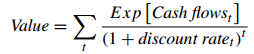
\includegraphics[width=90mm]{figures/formel1-1.png}
\caption{A simple caption \label{overflow}}
\end{figure}

If cash flow is riskless, future amount is always the same. If risky, depends on the state of the economy, olike how well business is doing.

Three ways to account for risk in the valuation procedure:
- Adjust the discount rate to a risk-adujusted discount rate. Reflects on time value of money and riskiness of cash flows. We can use Capital Asset Pricing Model (CAPM), or Arbitrage Pricing Theory /APT)
- Adjust risky cash flows so that they become certain cash flows that have the same value as risky ones. Can be calculated with CAPM or derivative securitires such as futures.
- Redefine the probabilities. Can use Black-Scholes-Merton Option Pricing. 



